\chapter{Introduction}
\section*{Abstract}
Here I give an overview on my thesis.
This includes:
\begin{itemize}
\item general topic
\item field of research: perceptual quality + judgment (relying on memorization and recall?)
\item relevance: why is this question relevant at all? Practical implications?
\item overview on service provider things: acceptance + satisfaction + money stuff
\item my personal motivation to tackle this topic (why important to me?)
\item how am I tackling the question?
\item what can the reader expect? (just hints)
\item (graphic) aspects of multi-episodic QoE: usage duration and time in between + usage pattern + multi-services
\end{itemize}

\section{Goal}
\begin{itemize}
\item How does perceptual quality evolve over multiple interactions (multiple episodes) with the one system/service for one user?
\item How does perceptual overall quality evolve over multiple interactions using a bundle, e.g. more than one system/service for one user? (basically an extension of previous stuff)
\item Goal 1: Find underlying effects temporal effects? (relate them to human memory)
\item Goal 2: Evaluate potential model components for temporal effects (Implement models: either service-independent (better) or service-dependent.)
\end{itemize}
%NOTE: Quality and model must be explained at least minimal here.

\begin{figure}
	\centering
	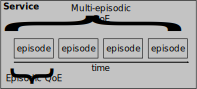
\includegraphics{fig/multi-episodic}
	\caption{Repeated usage episodes with one service and their episodic QoE form a multi-episodic QoE in the user.}
	\label{chap10:img:multiEpisodic}
\end{figure}

\section{Basic definitions}
\begin{itemize}
\item What is \emph{to service}? [Whitepaper] [http://www.merriam-webster.com/dictionary/service]
\item What is a service, application, system?
\item Telecommunication services + Service Provider
\end{itemize}

\paragraph*{Service provider's goal}
Make customer happy for as little money as possible for infrastructure: 
\begin{itemize}
\item cost-efficiency
\item risk reduction
\item Service usage
\item repeated usage / churn
\end{itemize}

\section{Aspects}
\begin{itemize}
\item QoE as hygienic factor [Moeller, Wechsung]  
\item Money: NPS, Churn, Acceptability, Willingness-to-paying
\item Retainability (sMOS)
\item Adaptive services: service that adjust performance to current conditions (best + economic feasible)
\end{itemize}

\section{Structure}
%TODO Here I describe the structure of my thesis    
